\documentclass[a4paper,11pt]{report}
\usepackage{chuan_math_gkt}
\usetikzlibrary{angles,quotes,intersections,patterns,decorations.pathreplacing}
\chuanexamsetup

\begin{document}
\examfontsize

\examsecret{绝密$\bigstar$启用前}

\examtitle{2020年普通高等学校招生全国统一考试（新课标III卷文科）}{数\quad 学}

\noticetitle
\begin{examnotice}
\item 答卷前，考生务必将自己的姓名、准考证号填写在答题卡上。
\item 回答选择题时，选出每小题的答案后，用铅笔把答题卡上对应题目的答案标号涂黑。如需改动，用橡皮擦干净后，再选涂其他答案标号。回答非选择题时，将答案写在答题卡上。写在本试卷上无效。
\item 考试结束后，将本试卷和答题卡一并交回。
\end{examnotice}
\examsection{一、选择题：本题共12小题，每小题5分，共60分。在每小题给出的四个选项中，只有一项是符合题目要求的。}
\begin{examquestions}

\item 已知集合A=\{1，2，3，5，7，11\}，B=\{x\textbar3< x<15\}，则A\ensuremath{\cap}B中元素的个数为

\fourchoices{2}{3}{4}{5}

\item 若$\overline{z}(1+i)=1-i$，则z=

\fourchoices{1-i}{1+i}{-i}{i}

\item 设一组样本数据$x_{1}$，$x_{2}$，\ensuremath{\ldots}，$x_{n}$的方差为0.01，则数据10$x_{1}$，10$x_{2}$，\ensuremath{\ldots}，10$x_{n}$的方差为

\fourchoices{0.01}{0.l}{1}{10}

\item Logistic模型是常用数学模型之一，可应用于流行病学领域，有学者根据公布数据建立了某地区新冠肺炎累计确诊病例数I(t)(t的单位：天)的Logistic模型：$I(t)=\dfrac{K}{1+e^{-0.23(t-53)}}$，其中K为最大确诊病例数。当I($t^{*}$)=0.95K时，标志着已初步遏制疫情，则$t^{*}$约为(ln19≈3)

\fourchoices{60}{63}{66}{69}

\item 已知sinθ+sin(θ+$\dfrac{\pi}{3}$)=1，则sin(θ+$\dfrac{\pi}{6}$)=

\onechoices{$\dfrac{1}{2}$}{$\dfrac{\sqrt{3}}{3}$}{$\dfrac{2}{3}$}{$\dfrac{\sqrt{2}}{2}$}

\item 在平面内，A，B是两个定点，C是动点，若$\vec{AC}\cdot\vec{BC}$=1，则C的轨迹为

\fourchoices{圆}{椭圆}{抛物线}{直线}

\item 设O为坐标原点，直线x=2与抛物线C：$y^{2}$=2px(p>0)交于D，E两点，若OD\ensuremath{\perp}OE，则C的焦点坐标为

\fourchoices{($\dfrac{1}{4}$，0)}{($\dfrac{1}{2}$，0)}{(1，0)}{(2，0)}

\item 点(0，1)到直线y=k(x+1)距离的最大值为

\fourchoices{1}{$\sqrt{2}$}{$\sqrt{3}$}{2}

\item 右图为某几何体的三视图，则该几何体的表面积是

\begin{tightcenter}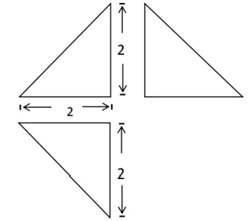
\includegraphics[width=2.17222in,height=1.92014in]{figures/2020_xkb3_wen_image14.png}\end{tightcenter}

\fourchoices{6+4$\sqrt{2}$}{4+4$\sqrt{2}$}{6+2$\sqrt{3}$}{4+2$\sqrt{3}$}

\item 设$a=\log_{3}2$，$b=\log_{5}3$，c=$\dfrac{2}{3}$，则

\fourchoices{a< c< b}{a< b< c}{b< c< a}{c< a< b}

\item 在\ensuremath{\triangle}ABC中，cosC=$\dfrac{2}{3}$，AC=4，BC=3，则tanB=

\fourchoices{$\sqrt{5}$}{2$\sqrt{5}$}{4$\sqrt{5}$}{8$\sqrt{5}$}

\item 已知函数f(x)=sinx+$\dfrac{1}{sinx}$，则

\onechoices{f(x)的最小值为2}{f(x)的图像关于y轴对称}{f(x)的图像关于直线x=π对称}{f(x)的图像关于直线x=$\dfrac{\pi}{2}$对称}

\item 著x，y满足约束条件\linsys{x+y\ensuremath{\geq}0\\2x-y\ensuremath{\geq}0\\x\ensuremath{\leq}1}，则z=3x+2y的最大值为
。

\item 设双曲线C：$\dfrac{x^{2}}{a^{2}}-\dfrac{y^{2}}{b^{2}}=1(a>0,b>0)$的一条渐近线为y=$\sqrt{2}$x，则C的离心率为
。

\item 设函数f(x)=$\dfrac{e^{x}}{x+a}$，若f\textquotesingle(1)=$\dfrac{e}{4}$，则a=
。

\item 已知圆锥的底面半径为1，母线长为3，则该圆锥内半径最大的球的体积为 。

\end{examquestions}
\examsection{三、解答题：共70分。解答应写出文字说明、证明过程或演算步骤。第17题～第21题为必考题，每个试题考生都必须作答。第22、23题为选考题，考生根据要求作答。}
\begin{examanswers}[start=17]


\item（12分）

设数列\{$a_{n}$\}满足$a_{1}$+$a_{2}$=4，$a_{3}$-$a_{1}$=8。

(1)求\{$a_{n}$\}的通项公式；

(2)记$S_{n}$为数列\{$\log_{3}a_{n}$\}的前n项和，若$S_{m}$+$S_{m+1}$=$S_{m+3}$，求m。

\item（12分）

某学生兴趣小组随机调查了某市100天中每天的空气质量等级和当天到某公园锻炼的人次，整理数据得到下表(单位：天)：

\begin{tightcenter}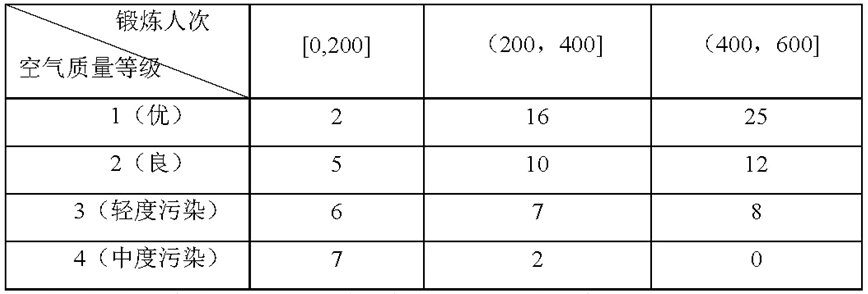
\includegraphics[width=5.76736in,height=1.95139in]{figures/2020_xkb3_wen_image27.png}\end{tightcenter}

(1)分别估计该市一天的空气质量等级为1，2，3，4的概率；

(2)求一天中到该公园锻炼的平均人次的估计值(同一组中的数据用该组区间的中点值为代表)；

(3)若某天的空气质量等级为1或2，则称这天``空气质量好''；若某天的空气质量等级为3或4，则称这天``空气质量不好''。根据所给数据，完成下面的$2\times2$列联表，并根据列联表，判断是否有95\%的把握认为一天中到该公园锻炼的人次与该市当天的空气质量有关?

\begin{tightcenter}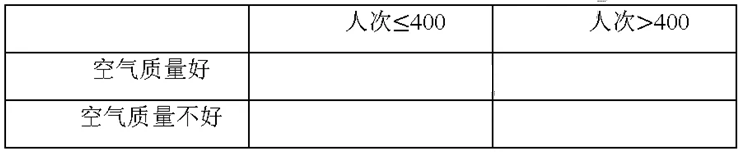
\includegraphics[width=5.75972in,height=1.21875in]{figures/2020_xkb3_wen_image28.png}\end{tightcenter}

附：$K^{2}=\dfrac{n(ad-bc)^{2}}{(a+b)(c+d)(a+c)(b+d)}$

\begin{tightcenter}
\begin{tabular}{|c|c|c|c|}\hline
$P(K^2\ensuremath{\geq} k)$ & 0.050 & 0.010 & 0.001\\ \hline
$k$ & 3.841 & 6.635 & 10.828\\ \hline
\end{tabular}
\end{tightcenter}

\item（12分）

如图，在长方体ABCD-$A_{1}$$B_{1}$$C_{1}$$D_{1}$中，点E，F分别在棱D$D_{1}$，B$B_{1}$上，且2DE=E$D_{1}$，BF=2F$B_{1}$。证明：

\begin{tightcenter}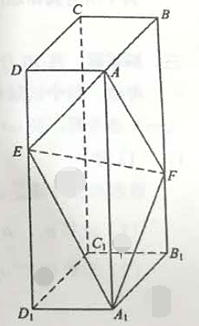
\includegraphics[width=1.22708in,height=2.01111in]{figures/2020_xkb3_wen_image31.png}\end{tightcenter}

(1)当AB=BC时，EF\ensuremath{\perp}AC；

(2)点$C_{1}$在平面AEF内。

\item（12分）

己知函数f(x)=$x^{3}$-kx+$k^{2}$。

(1)讨论f(x)的单调性；

(2)若f(x)有三个零点，求k的取值范围。

\item（12分）

已知椭圆C：$\dfrac{x^{2}}{25}+\dfrac{y^{2}}{m^{2}}=1(0<m<5)$的离心率为$\dfrac{\sqrt{15}}{4}$，A，B分别为C的左、右顶点。

(1)求C的方程；

(2)若点P在C上，点Q在直线x=6上，且\textbar BP\textbar=\textbar BQ\textbar，BP\ensuremath{\perp}BQ，求\ensuremath{\triangle}APQ的面积。


\item（10分）

{[}选修4-4：坐标系与参数方程{]}(10分)

在直角坐标系xOy中，曲线C的参数方程为\linsys{x=2-t-t^{2}\\y=2-3t+t^{2}}(t为参数且t\ensuremath{\ne}1)，C与坐标轴交于A，B两点。

(1)求\textbar AB\textbar；

(2)以坐标原点为极点，x轴正半轴为极轴建立极坐标系，求直线AB的极坐标方程。

\item（10分）

{[}选修4-5：不等式选讲{]}(10分)

设a，b，c\ensuremath{\in}R，a+b+c=0，abc=1。

(1)证明：ab+bc+ca<0；

(2)用max\{a，b，c\}表示a，b，c的最大值，证明：max\{a，b，c\}\ensuremath{\geq}$\sqrt[4]{3}$。
\end{examanswers}

\end{document}
